% Editable source for design.pdf (pdflatex design.tex). Schematic; widths are not to scale.
% The measured Bernstein-Lange arm: budget matching, the shared walk, and the per-target arms.
\documentclass[tikz,border=6pt]{standalone}
\usepackage[T1]{fontenc}
\usetikzlibrary{positioning,arrows.meta,decorations.pathreplacing,backgrounds}
\begin{document}
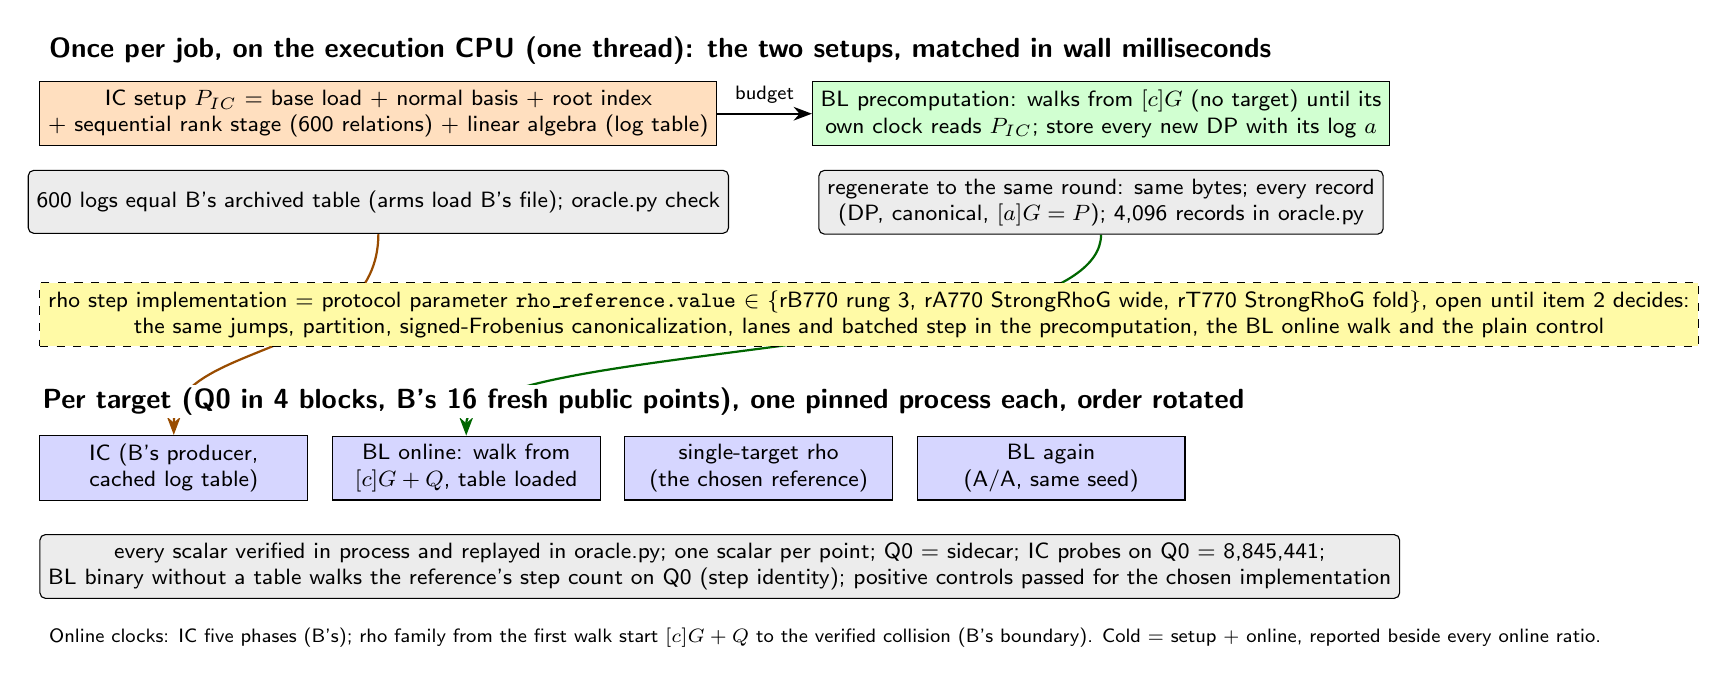
\begin{tikzpicture}[font=\sffamily\footnotesize,>=Stealth,
  box/.style={draw,minimum height=8mm,inner sep=3pt,align=center},
  once/.style={box,fill=orange!25},
  bl/.style={box,fill=green!18},
  online/.style={box,fill=blue!16},
  check/.style={box,fill=gray!15,rounded corners=2pt},
  open/.style={box,fill=yellow!35,dashed}]
% Row 1: the two setups, matched in the same unit.
\node[anchor=west,font=\sffamily\bfseries] at (0,6.0) {Once per job, on the execution CPU (one thread): the two setups, matched in wall milliseconds};
\node[once,minimum width=70mm,anchor=west] (ic) at (0,5.2) {IC setup $P_{IC}$ = base load + normal basis + root index\\+ sequential rank stage (600 relations) + linear algebra (log table)};
\node[bl,minimum width=70mm,right=12mm of ic] (pre) {BL precomputation: walks from $[c]G$ (no target) until its\\own clock reads $P_{IC}$; store every new DP with its log $a$};
\draw[->,thick] (ic.east) -- node[above,font=\sffamily\scriptsize]{budget} (pre.west);
\node[check,minimum width=70mm,below=3mm of ic] (icck) {600 logs equal B's archived table (arms load B's file); oracle.py check};
\node[check,minimum width=70mm,below=3mm of pre] (preck) {regenerate to the same round: same bytes; every record\\(DP, canonical, $[a]G=P$); 4,096 records in oracle.py};
% Row 2: the walk is one object.
\node[open,minimum width=146mm,anchor=west] (impl) at (0,2.65) {rho step implementation = protocol parameter \texttt{rho\_reference.value} $\in$ \{rB770 rung 3, rA770 StrongRhoG wide, rT770 StrongRhoG fold\}, open until item 2 decides:\\the same jumps, partition, signed-Frobenius canonicalization, lanes and batched step in the precomputation, the BL online walk and the plain control};
% Row 3: per target arms.
\node[anchor=west,font=\sffamily\bfseries,fill=white,inner sep=1pt] at (0,1.55) {Per target (Q0 in 4 blocks, B's 16 fresh public points), one pinned process each, order rotated};
\node[online,minimum width=34mm,anchor=west] (a1) at (0,0.7) {IC (B's producer,\\cached log table)};
\node[online,minimum width=34mm,right=3mm of a1] (a2) {BL online: walk from\\$[c]G+Q$, table loaded};
\node[online,minimum width=34mm,right=3mm of a2] (a3) {single-target rho\\(the chosen reference)};
\node[online,minimum width=34mm,right=3mm of a3] (a4) {BL again\\(A/A, same seed)};
\begin{scope}[on background layer]
\draw[->,thick,green!40!black] (preck.south) .. controls +(0,-1.6) and +(0,1.2) .. (a2.north);
\draw[->,thick,orange!60!black] (icck.south) .. controls +(0,-1.6) and +(0,1.2) .. (a1.north);
\end{scope}
\node[check,minimum width=146mm,anchor=west] (gates) at (0,-0.55) {every scalar verified in process and replayed in oracle.py; one scalar per point; Q0 = sidecar; IC probes on Q0 = 8,845,441;\\BL binary without a table walks the reference's step count on Q0 (step identity); positive controls passed for the chosen implementation};
\node[anchor=west,font=\sffamily\scriptsize,align=left] at (0,-1.45) {Online clocks: IC five phases (B's); rho family from the first walk start $[c]G+Q$ to the verified collision (B's boundary). Cold = setup + online, reported beside every online ratio.};
\end{tikzpicture}
\end{document}
